
Wie bereits in \cref{sec:int} erwähnt, wollen wir uns zunächst mit dem genauen
Verhältnis einer reinen Quinte ($2:3$) beschäftigen. Die Differenz zur
gleichstufigen Quinte, nämlich
\[1{,}200\,\on{ct}\cdot \log_2(\tfrac32) - 700\,\on{ct} \approx 1.96\,\on{ct}\]%
wird manchmal auch \emph{Grad} genannt\todo{Man müsste eigentlich irgendwo mal sagen, dass das Grad $\frac{1}{12}$ des Pyth. Kommas ist. Und dass 12-EDO genau das tut: Das Pyth. Komma auf 12 Quinten aufteilen. –T}
und ist sehr klein, aber dennoch etwas das wir korrigieren wollen. Ohne die
Einschränkungen eines Instruments mit diskreten Tonhöhen kann dies leicht
erreicht werden, wenn wir akzeptieren, dass enharmonisch unterschiedene
Tonhöhen verschiedenen Frequenzen entsprechen können.

Dies mag auf den ersten Blick seltsam erscheinen, aber man kann sich davon
überzeugen, indem man eine übermäßige Sekunde (in einem angemessenen
harmonischen Kontext) mit einer kleinen Terz vergleicht und versucht, sie zu
singen: Wir sehen keinen Grund, warum sie genau das gleiche Frequenzverhältnis
haben sollten. Ein weiteres eindrucksvolles Beispiel ist in
\cref{fig:enhContext} zu sehen (das Audiobeispiel ist in gleichstufiger
Stimmung): In beiden Fällen ist das resultierende Intervall acht \acr{HTS} groß
(\flat e’\,-\,h’ und \sharp d’\,-\,h’), aber im ersten Fall klingt es
dissonant, da der Kontext nahelegt, dass es aus vier Ganztönen besteht, während
es im zweiten Fall konsonant klingt.

\begin{figure}[h]
  \centering
  \LY{b-enhContext}
  \includegraphics{ly/b-enhContext.pdf}
  \caption{Eine übermäßige Quinte ist keine kleine Sexte.}\label{fig:enhContext}
\end{figure}

Akzeptierend, dass Enharmonik eine Rolle spielt, machen wir uns die Tatsache
zunutze, dass es für jede enharmonisch verschiedene Tonhöhe (c’, \sharp h und
\dflat d’ sind drei unterschiedliche Beispiele!) eindeutig bestimmte ganze
Zahlen $p,q\in\Z$ gibt, so dass die Tonhöhe von a’ aus erreicht werden kann,
indem man $p$ reine Quinten und $q$ Oktaven nach oben geht (eine negative Zahl
bedeutet, dass man nach unten geht). Setzen wir den Kammerton auf $440\Hz$, so
ordnen wir der Tonhöhe die Frequenz $(\frac32)^p\cdot 2^q\cdot 440\Hz$ zu. Ein
Beispiel:\looseness-1
\begin{align*}
  \text{\sharp g’}&\equiv(\tfrac32)^5\cdot 2^{-3}\cdot 440\Hz\approx 417.66\Hz\\
  \text{\flat a’} &\equiv(\tfrac32)^{-7}\cdot 2^4\cdot 440\Hz\approx 412.03\Hz
\end{align*}
Der Unterschied zwischen diesen beiden Frequenzen heißt
\emph{pythagoreisches Komma} und ist
$3^{12}\cdot 2^{-19}\approx 23.46\,\on{ct}$. Eine verminderte Sexte
unterscheidet sich von einer reinen Quinte notwendigerweise um genau dieses
pythagoreische Komma. Eine verminderte Sexte wird in der pythagoreischen
Stimmung manchmal als „Wolfsintervall“ bezeichnet, da sie sehr verstimmt
klingt, siehe \cref{fig:pythComma}. In \cref{fig:spiral5}, ist eine
enharmonische Variante des Quintenzirkels zu sehen, die wir als
\emph{Quintenspirale} bezeichnen können. Mit jeder vollen Runde in dieser
Spirale, verschiebt sich die Tonhöhe um ein pythagoreisches Komma.\todo{Hier ein Wort zu Skalen?}

\begin{figure}[h]
  \centering
  \includegraphics{ly/b-pythComma}
  \LY{b-pythComma}
  \caption{(1) Der Unterschied zwischen \sharp g’ and \flat a’. (2) Das
    Wolfsintervall \sharp g’\,–\,\flat e’, gefolgt von der reinen Quinte \sharp
    g’\,–\,\sharp d’.}\label{fig:pythComma}
\end{figure}

Für jedes Intervall können wir das entsprechende Verhältnis berechnen, siehe
\cref{tab:1}. Man beachte, dass, wenn ein bestimmtes Intervall das Verhältnis
$a:b$ hat, sein \emph{Komplementärintervall} das Verhältnis $b:2a$ hat, z.\,B.\
eine kleine Sexte entspricht dem Verhältnis $81:128$. Ähnlich verhält es sich,
wenn ein Intervall die Größe $c$ in Cent hat: Dann hat sein
Komplementärintervall die Größe $1{,}200\,\on{ct}-c$, z.\,B. eine kleine Sexte
entspricht $792.18\,\on{ct}$.

\begin{figure}
  \centering%
  \newcommand{\pitcharray}{%
  \dflat D, \dflat A, \dflat E, \dflat B, \flat F,
  \flat C, \flat G, \flat D, \flat A, \flat E,
  \flat B, F, C, G, D, A, E, B,
  \sharp F, \sharp C, \sharp G, \sharp D, \sharp A, \sharp E, \sharp B}
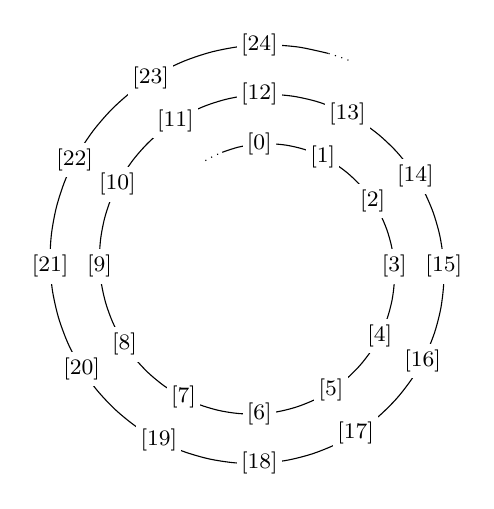
\begin{tikzpicture}[xscale=-1]
  \def\xA{1.4}
  \def\xB{.1}
  \draw[dotted,domain=.35*pi:.4*pi,smooth,samples=100,variable=\t]
  plot ({(\xA+\xB*\t)*cos(\t r)},{(\xA+\xB*\t)*sin(\t r)});
  \draw[domain=.4*pi:4.6*pi,smooth,samples=100,variable=\t]
  plot ({(\xA+\xB*\t)*cos(\t r)},{(\xA+\xB*\t)*sin(\t r)});
  \draw[dotted,domain=4.6*pi:4.63*pi,smooth,samples=100,variable=\t]
  plot ({(\xA+\xB*\t)*cos(\t r)},{(\xA+\xB*\t)*sin(\t r)});
  \foreach \i in {0,...,24}{
    \node[fill=white,inner sep=1.5px]
    at ({(\xA+\xB*(\i+3)*pi/6)*cos((\i+3)*pi/6 r)},
    {(\xA+\xB*(\i+3)*pi/6)*sin((\i+3)*pi/6 r)})
    {\footnotesize \pitch[\i]$\strut$};
  };
\end{tikzpicture}

  \caption{Die enharmonische Quintenspirale. Mit jeder vollen Rotation im
  	Uhrzeigersinn, gewinnen wir ein pythagoreisches Komma.}\label{fig:spiral5}
\end{figure}

\begin{table}
  \centering
  \begin{tabular}{lr@{\hspace*{2.4px}}lr}
    \toprule
    \textsc{Intervall} & \multicolumn{2}{c}{\textsc{Verhältnis}} & \textsc{Größe in ct}\\
    \midrule
    kleine Sekunde  & $243$ & $:256$ &  $90.22$\\
    große Sekunde   & $8$   & $:9$   & $203.91$\\
    kleine Terz     & $27$  & $:32$  & $294.13$\\
    große Terz      & $64$  & $:81$  & $407.82$\\
    reine Quarte    & $3$   & $:4$   & $498.04$\\
    \bottomrule
  \end{tabular}
  \caption{Ausgewählte Intervalle in pythagoreischer Stimmung.}\label{tab:1}
\end{table}

Von nun an interpretieren wir geschriebene Noten in pythagoreischer
Stimmung und bezeichnen alle Abweichungen davon mit bestimmten Symbolen, die
wir einführen, wenn sie notwendig werden. Man beachte jedoch, dass der
Unterschied zu der gleichstufigen Stimmung eher gering ist.\todo{(Außer man schreibt verrückte Sachen wie \dflat h und \dsharp g. Die unterscheiden sich in 12-EDO nicht, aber in pyth. Stimmung um $46.9\,\on{ct}$.) –T}
Während alle noch kommenden Mikroalterationen (die darauf abzielen, ganze
Akkorde zu stimmen) den Preis haben werden, dass es mehrere Frequenzen für
denselben Tonnamen gibt, verwendet die bare pythagoreische Stimmung nur die
Informationen, die uns durch die geschriebenen Noten gegeben werden. Sie verhält
sich aus \emph{melodischer} Perspektive also gut™, da die Größe der 
(horizontalen) Intervalle nicht von der vertikalen Struktur abhängt.\todo{Also ein Beweis ist das nicht, oder? Falsche Schlussrichtung oder so … Einen Grund dafür, dass pythagoreische Stimmung für sinnvolle Melodien sorgt, habe ich in der Rotation des Mikrotöne-Kurses auf der zweiten Hälfte vorgeführt bekommen: In pythagoreischer Stimmung gibt es \emph{diatonische} Skalen, also Skalen die nur zwei unterschiedliche Schrittweiten haben (i.e. Halbton und Ganzton). In der Rotation hat Georg so ein 22-EDO Beispiel vorgespielt mit $\acr{GT}:\acr{HT} = 4:1$. Das Beispiel produziert grauenhafte Dreiklänge, aber eine Tonleiter mit LLSLLLS hörte sich relativ melodisch an und war eindeutig Dur. –T}

Der einzige Nachteil der pythagoreischen Stimmung, der nichts mit der
Realisierbarkeit auf einem diskretisierenden Instrument zu tun hat, sondern rein
theoretisch ist, ist die Tatsache, dass sie die Unreinheit der Terzen in einem
Dreiklang im Vergleich zur gleichstufigen Stimmung sogar noch erhöht: Der
Unterschied zwischen einer pythagoreischen großen Terz ($407.82\,\on{ct}$) und
dem oben erwähnten Verhältnis $4:5$ ($386.31\,\on{ct}$) beträgt
$21.51\,\on{ct}$. Dieser Fehler ist Gegenstand des nächsten Abschnitts.

% We close this section by considering a three harmonic situations, which could
% appear in western classical music and which require enharmonic sensitivity, see
% \cref{fig:reint}: In the first case, we have a dominant seventh in \flat E major,
% leading to the tonic, while in the second case, we see the German augmented
% sixth chord (which might be seen as a variation of a dominant chord based on E),
% leading to A major. The third example shows how a diminished seventh chord can
% be enharmonically reinterpreted: It is introduced as the dominant of A minor,
% but then reinterpreted as the dominant of C minor, leading to the new tonic. We
% play these chords in Pythagorean tuning.

% \begin{figure}[h]
%   \centering%
%   \includegraphics{ly/b-reint.pdf}%
%   \LY{b-reint}%
%   \caption{Three situations showing the different rôles of \sharp G and \flat
%     A.}\label{fig:reint}
% \end{figure}

%%% Local Variables:
%%% mode: latex
%%% TeX-master: "../main"
%%% End:
